\pdfminorversion=5      %~ Version 1.5 of the PDF specification
\pdfobjcompresslevel=2  %~ compression of non-stream objects

\documentclass[
    t,
    smaller,
    compress,
    xcolor=svgnames,            %~ named colors
    table,
]{beamer}
\usepackage[utf8]{inputenc}
\usepackage[ngerman]{babel}

\usepackage{listings}

% --- Farbdefinitionen ---------------------------------------------------------
\definecolor{dkgreen}{rgb}{0,0.6,0}
% Solarized palette (modified)
\definecolor{solarized@base03}{HTML}{002B36}
\definecolor{solarized@base02}{HTML}{073642}
\definecolor{solarized@base01}{HTML}{384ea5}
\definecolor{solarized@base00}{HTML}{657b83}
\definecolor{solarized@base0}{HTML}{839496}
\definecolor{solarized@base1}{HTML}{93a1a1}
\definecolor{solarized@base2}{HTML}{EEE8D5}
\definecolor{solarized@base3}{HTML}{FDF6E3}
\definecolor{solarized@yellow}{HTML}{754900}
\definecolor{solarized@orange}{HTML}{CB4B16}
\definecolor{solarized@red}{HTML}{DC322F}
\definecolor{solarized@magenta}{HTML}{D33682}
\definecolor{solarized@violet}{HTML}{6C71C4}
\definecolor{solarized@blue}{HTML}{268BD2}
\definecolor{solarized@cyan}{HTML}{0A8178}
\definecolor{solarized@green}{HTML}{657900}

\lstset{language=Python,
  basicstyle=\ttfamily,
  numberstyle=\tiny\color{solarized@base01},
  keywordstyle=\color{solarized@green},
  stringstyle=\color{solarized@cyan},
  identifierstyle=\color{solarized@base03},
  commentstyle=\color{solarized@base01},
  emphstyle=\color{solarized@red},
  procnamestyle=\color{solarized@blue}\textbf,
  backgroundcolor=\color{White},
  rulesepcolor=\color{solarized@base1},
  tabsize=4,
  columns=fullflexible,
  keepspaces=true,
  breaklines=true,
  breakatwhitespace=true,
  showstringspaces=false,
  extendedchars=true%
}
\lstdefinestyle{Java} {language=Java}

\usetheme{BerlinFU}
\setbeamercolor{postit}{fg=black, bg=solarized@base3}

%~ \usefonttheme{professionalfonts}
%~ \usepackage[noae]{Sweave}


\hypersetup{pdfstartview={FitH}} % By default the pdf fit the width of the screen.
%~ \hypersetup{pdfpagemode=FullScreen}


% http://tex.stackexchange.com/questions/16357/how-can-i-position-an-image-in-an-arbitrary-position-in-beamer
\usepackage{tikz}
\tikzset{
  every overlay node/.style={
    anchor=north west,
  },
}
% Usage:
% \tikzoverlay at (-1cm,-5cm) {content};
% or
% \tikzoverlay[text width=5cm] at (-1cm,-5cm) {content};
\def\tikzoverlay{%
   \tikz[baseline,overlay]\node[every overlay node]
}%


% http://tex.stackexchange.com/questions/48473/best-way-to-give-sources-of-images-used-in-a-beamer-presentation
\usepackage[absolute,overlay]{textpos}

\setbeamercolor{framesource}{fg=gray}
\setbeamerfont{framesource}{size=\footnotesize}


%%% inline todonotes %%%%%%%%%%%%%%%%%%%%%%%%%%%%%%%%%%%%%%%%%%%%%%%%%%%%%%%%%%
\usepackage{todonotes}
%\usepackage[disable]{todonotes} % Hide notes
\presetkeys{todonotes}{inline}{}


%%% Macros %%%%%%%%%%%%%%%%%%%%%%%%%%%%%%%%%%%%%%%%%%%%%%%%%%%%%%%%%%%%%%%%%%%%
\newcommand{\source}[1]{
    \vspace{-4pt}
    \begin{beamercolorbox}[ht=4pt,right]{framesource}
        \usebeamerfont{framesource}\usebeamercolor[fg]{framesource} Quelle: {#1}
    \end{beamercolorbox}
}

%% POSTIT
\newenvironment{beamerpostit}[1]%%
{\begin{beamercolorbox}[wd=\textwidth,sep=2pt,rounded=true,shadow=true]{postit} #1}%
{\end{beamercolorbox}}%


\defbeamertemplate*{section in toc}{my theme}
{\leavevmode\leftskip=0em\large{\usebeamercolor[fg]{titlelike}\inserttocsectionnumber.} \inserttocsection\par\vspace{10pt}}

\defbeamertemplate*{subsection in toc}{my theme}
{\leavevmode\leftskip=2em\normalsize{\usebeamercolor[fg]{titlelike}\inserttocsectionnumber.\inserttocsubsectionnumber.} \inserttocsubsection\par}

\defbeamertemplate*{subsubsection in toc}{my theme}
{\leavevmode\leftskip=3.5em\normalsize\usebeamerfont{subsection in toc}\usebeamerfont{subsubsection in toc}\inserttocsubsubsection\par}


%%% Formatting table %%%%%%%%%%%%%%%%%%%%%%%%%%%%%%%%%%%%%%%%%%%%%%%%%%%%%%%%%%%
\usepackage{booktabs, colortbl, tabularx}


%% PLOT %%%%%%%%%%%%%%%%%%%%%%%%%%%%%%%%%%%%%%%%%%%%%%%%%%%%%%%%%%%%%%%%%%%%%%%%
%\usetikzlibrary{shapes, intersections, calc, backgrounds}
%% Ploting
%\usepackage{pgfplots}
%\usepackage{pgfplotstable}


%~ Anzahl Folien: pro Folie solltet ihr mindestens 90s einplanen
%~
%~ Übergänge roter Faden
%~
%~ Konzept Vortrag

%~ TODO
%~ Eventuell Python Handout


%~ \begin{frame}
  %~ \frametitle{}
  %~ \begin{columns}[T]
    %~ \begin{column}{.5\textwidth}<1->
      %~
    %~ \end{column}
    %~ \begin{column}{.5\textwidth}<1->
      %~ \begin{figure}
        %~ \includegraphics[height=40mm]{}
        %~ \source{[\ref{}]}
      %~ \end{figure}
    %~ \end{column}
  %~ \end{columns}
%~ \end{frame}


%% BIBLIOGRAPHY %%%%%%%%%%%%%%%%%%%%%%%%%%%%%%%%%%%%%%%%%%%%%%%%%%%%%%%%%%%%%%%%

%~ don't span the whole text width in the bibliography.
%\usepackage[style=alphabetic]{biblatex}
%~ expects reference database file named "references.bib"
%\bibliography{references}
%\DeclareFieldFormat{formaturl}{\iffieldundef{url}{}{\newline #1}}
%\renewbibmacro{url+urldate}{\printtext[formaturl]{\printfield{url}}}


\newlength\yearposx


\title{Webframeworks für Python}
\subtitle{Vorstellung und Vergleich}
\author{Andreas Knöpfle, Bastien Sachs und Tobias Schmid}
\institute{Institut für Informatik}
\date{28.\,November 2012}
%~ \titlegraphic{silberlaube2}


\begin{document}


{
\setbeamertemplate{footline}{}
\begin{frame} % Titelseite
    \titlepage
\end{frame}
}


\begin{frame}
  %\frametitle{}
  Einstiegs-Idee:\\
  viele Logos der Webframeworks für Python\\
  Stichpunkte:\\
   - In Python geschriebene Webframework gibt es wie „Sand am Meer“\\
   - Warum? Einblick gibt unser Vortrag\\

  %~ Größe spiegelt „Machtverhältnisse“ da
  %~ Einige werdet ihr im Laufe des Vortrages kennenlernen
  %~ Hat jemand schon von einem Webframework für Python gehört?
\end{frame}


\begin{frame}
  \frametitle{Gliederung}
  \tableofcontents
  %~ roter Faden
\end{frame}


\section{Python~-- Programmiersprache fürs Web?}

\subsection{Philosophie}
\begin{frame}
  \frametitle{Python~-- Programmiersprache fürs Web?}

  % 1991 erstmals erschienen, aktuelle Versionen: 3.3.0 (September 2012), 2.7.3 (April 2012)
  % http://en.wikipedia.org/wiki/History_of_Python
  \vspace{12pt}
  \begin{tikzpicture}[scale=0.48] % timeline 1991-2012->
    % define coordinates (begin, used, end, arrow)
    \foreach \x in {1991,1994,2004,2008,2012,2013}{
        \pgfmathsetlength\yearposx{(\x-1991)*1cm};
        \coordinate (y\x)   at (\yearposx,0);
        \coordinate (y\x t) at (\yearposx,+3pt);
        \coordinate (y\x b) at (\yearposx,-3pt);
    }

    % draw horizontal line with arrow
    \draw [->] (y1991) -- (y2013);

    % draw ticks
    \foreach \x in {1991,1994,2004,2008,2012}
        \draw (y\x t) -- (y\x b);

    % annotate (draw nodes)
    \foreach \x in {1991,1994,2004,2008,2012}
        \node at (y\x) [below=3pt] {\x};

    \node at (6.5cm, 2.5cm) {\pgftext{
\includegraphics[height=1cm]{python_1990.png}}};
    \node at (18cm, 2.5cm) {\pgftext{
\includegraphics[height=1cm]{python_logo_2006.png}}};

    \fill (y1991) circle (3pt) node[above=3pt] {0.9};
    \fill (y1994) circle (3pt) node[above=3pt] {1.0};
    \fill (y2004) circle (3pt) node[above=3pt] {2.0};
    \fill (y2008) circle (3pt) node[above=3pt] {3.0};
    \fill (y2012) circle (3pt) node[above=3pt] {2.7.3, 3.3.0};
  \end{tikzpicture}
  \vspace{12pt}

  \begin{itemize}[<1->]
    \item Entwurfsphilosophie betont Programmlesbarkeit
    \begin{itemize}[<1->]
      \item Blöcke durch gleiche Einrückung begrenzt
      \item relativ wenige Schlüsselwörter
    \end{itemize}
    %\item Dynamische Programmiersprache
   % Python-Interpreter mit interaktiven Modus
    \item Multiparadigmen-Sprache (primär OOP, funktional, AOP)
    \item dynamische Datentypen, garbage collection
    \item große, umfangreiche Standardbibliothek “batteries included”
  \end{itemize}

 %~ The Zen of Python http://www.python.org/dev/peps/pep-0020/
 %~ http://brainsik.theory.org/.:./2009/why-reddit-uses-python
 %~ http://www.quora.com/Quora-Infrastructure/Why-did-Quora-choose-Python-for-its-development

  %~  * Plugins für Eclipse, NetBeans, Vim, Emacs und v.a.
\end{frame}


%\begin{frame}
%
%  \hspace{12pt}
%  \makebox[\textwidth][c]{%
%    \begin{minipage}[c]{0.85\columnwidth}
%      \resizebox{\linewidth}{!}{PEP 8}
%    \end{minipage}
%  }
%  %~ coding conventions
%
%\end{frame}


%~ Codebeispiele
%~ Gegenüberstellungen mit schon behandelten Sprachen
\subsection{Plattformvergleich}
\begin{frame}[fragile]
  \frametitle{Syntaxvergleich zu Java}
  \vspace{-12pt}

  \begin{columns}[T]
    \begin{column}{.8\textwidth}<1->
      \begin{lstlisting}[style=Java]
int value = 0;
String title = String.valueOf(value);
if ("0".equals(title)) {
    throw new Exception("Error");
}
for (int i = 1; i < 10; i++) {
    System.out.printf("row %s", i);
}
      \end{lstlisting}
    \end{column}
    \begin{column}{.2\textwidth}<1->
      \begin{figure}
        
\includegraphics[height=25mm]{java_logo.png}
        \source{[\ref{illu:2}]}
      \end{figure}
    \end{column}
  \end{columns}

  \vspace{12pt}

  \begin{columns}[T]
    \begin{column}{.8\textwidth}<1->
      \begin{lstlisting}
value = 0
title = str(value)
if title == "0":
    raise Exception("Error")
for i in range(1, 10):
    print "row {}".format(i)
      \end{lstlisting}
    \end{column}
        \begin{column}{.2\textwidth}<1->
      \begin{figure}
        
\includegraphics[height=25mm,trim=0 0 1500px 0]{python_logo_2006.png}
        \source{[\ref{illu:2}]}
      \end{figure}
    \end{column}
  \end{columns}

  %~ * Development style issues
\end{frame}


\begin{frame}[fragile]
  \frametitle{Softwarequalität im Plattformvergleich}

  \rowcolors{1}{white}{solarized@base3}
  \begin{table}[h]
    \begin{tabular}{|l||c|c|c|}
     \hline
      Eigenschaft          & \cellcolor{dkgreen} + & \cellcolor{yellow} & \cellcolor{red} - \\ \hline \hline

      Aufwand   & \textbf{Python} & Ruby & Java, PHP  \\ \hline
      Lesbarkeit           & \textbf{Python} & Ruby & Java, PHP \\ \hline
      %~ http://de.wikipedia.org/wiki/Modifizierbarkeit
      Modifizierbarkeit    & \textbf{Python} & Ruby & Java, PHP \\ \hline
      %~ http://de.wikipedia.org/wiki/Robustheit
      Robustheit           & Java, \textbf{Python}, Ruby & -- & PHP \\ \hline
      Sicherheit           & Java, \textbf{Python}, Ruby & -- & PHP \\ \hline
      %~ http://de.wikipedia.org/wiki/Programmierwerkzeug
      Werkzeuge & Java & PHP, \textbf{Python}, Ruby &  \\ \hline
    \end{tabular}
  \end{table}

  Ähnliche/sekundäre Eigenschaften: Abhängigkeit von Programmierwerkzeugen,
  Skalierbarkeit und Speicherbedarf

  \vspace{12pt}
  Vereinfachte Übersicht auf Grundlage von %\citetitle{hardy:2007} %\cite{hardy:2007}
\end{frame}


\subsection{Portabilität durch WSGI}
\begin{frame}
  \frametitle{Web Server Gateway Interface (WSGI)}
  %~ http://www.python.org/dev/peps/pep-0333/
  %~ http://wsgi.readthedocs.org/en/latest/
  %~ http://www.ibm.com/developerworks/library/wa-wsgi/
  %~ http://de.wikipedia.org/wiki/Web_Server_Gateway_Interface
  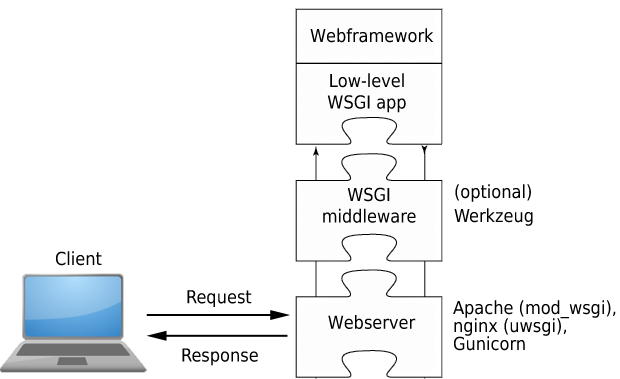
\includegraphics[height=60mm]{wsgi.png}
\end{frame}


\begin{frame}
  \frametitle{Python~-- Programmiersprache fürs Web!}

  Zusammenfassung der genannten Punkte

  \todo{add bullet points, aber dann auch mit Argumentation warum
      das für Webanwendungen besonders geeignet ist ==$>$ B.}

\end{frame}


\section{Webframeworks für Python}
\begin{frame}
  \frametitle{Webframeworks für Python (Auswahl)}
  %~ TODO add logos

  \begin{columns}[T]
    \begin{column}[T]{.5\textwidth}<1->
        Full-Stack Frameworks
        \vspace{4pt}
        \begin{itemize}[<1->]
            \item \textbf{Django}
            \item \textbf{TurboGears}
            \item web2py
            \item Pylons/Pyramid
            \item \dots
        \end{itemize}
    \end{column}
    \begin{column}[T]{.5\textwidth}<1->
        Microframeworks
        \begin{itemize}[<1->]
            \item \textbf{Bottle}
            \item \textbf{Tornado}
            \item \textbf{Flask}
            \item \textbf{web.py}
            \item CherryPy
            \item \dots
        \end{itemize}
    \end{column}
  \end{columns}

% , Other Full-Stack Frameworks, Basic Frameworks
% * Django\\
% * CherryPy, CubicWeb, Flask, Grok, Plone, Pylons, %Pyramid, TurboGears, web2py, Zope 2\\
% * Bottle, Karrigell, Nagare, Pyjamas, Quixote, Spyce, %Tornado, TwistedWeb, Web.py\\
% * Nicht mehr aktiv: Albatross, BlueBream, Nevow, Webware\\
\end{frame}


\subsection{Django}
\begin{frame}
  \begin{figure}
                    
\includegraphics[width=25mm]{django-logo.png}
                    \source{[\ref{illu:9}]}
  \end{figure}

  \begin{beamerpostit}
    \begin{quote}
      “The web framework for perfectionists with deadlines”
    \end{quote}
  \end{beamerpostit}

  \vspace{12pt}
  \begin{tikzpicture}[scale=0.88] % timeline 2003-2012->
    % define coordinates (begin, used, end, arrow)
    \foreach \x in {2003,2005,2008,2012,2013}{
        \pgfmathsetlength\yearposx{(\x-2003)*1cm};
        \coordinate (y\x)   at (\yearposx,0);
        \coordinate (y\x t) at (\yearposx,+3pt);
        \coordinate (y\x b) at (\yearposx,-3pt);
    }

    % draw horizontal line with arrow
    \draw [->] (y2003) -- (y2013);

    % draw ticks
    \foreach \x in {2003,2008,2012}
        \draw (y\x t) -- (y\x b);

    % annotate (draw nodes)
    \foreach \x in {2003,2005,2008,2012}
        \node at (y\x) [below=3pt] {\x};

    \fill (y2005) circle (3pt) node[above=3pt] {0.9};
    \fill (y2008) circle (3pt) node[above=3pt] {1.0};
    \fill (y2012) circle (3pt) node[above=3pt] {1.4.2};
  \end{tikzpicture}
  \vspace{12pt} \\
  Wichtige Designprinzipien:
  \begin{itemize}[<1->]
  \item Don’t repeat yourself (DRY)
  \item Explicit is better than implicit
  \end{itemize}
  %~ Some well known sites that use Django include Pinterest, Instagram, Mozilla,
  %~ The Washington Times and the Public Broadcasting Service.

\end{frame}


\subsection{Vergleichskriterien}
\begin{frame}
Hauptteil:\\
Vor- und Nachteile einiger weniger Frameworks aufzeigen\\
(konkrete) Lösungsansätze für bestimmte Probleme/Vergleichskriterien
\todo{Aber schon entlang aller Kriterien.}

    \frametitle{Farbdeutung bei Vergleichen}

    \todo{Testen Sie bitte mit dem Beamer ob das Orange vom Rot unterscheidbar ist.}
    \begin{table}[h]
        \begin{tabular}{|c|}
            \hline
             \cellcolor{dkgreen} sehr gute Lösung  \\ \hline
            \cellcolor{orange} in manchen Fällen evtl. nicht optimal \\ \hline
            \cellcolor{red} nicht optimale Lösung \\ \hline
         \end{tabular}
    \end{table}

\end{frame}


%~ MVC (Model-View-Controller) design paradigm


\begin{frame}
  \frametitle{Persistenz}

    \textbf{SQL-ORMs}
    \begin{itemize}[<1->]
        \item Django built-in ORM (Django)
        \item SQLAlchemy (Pylons,Turbogears) %Gork,Zope
        % \item Storm (Grok )
        \item SQLObject (Pylons,TurboGears)
        \item DAL (web2py)
        \item \dots
     \end{itemize}
     \textbf{MongoDB ORMs}
    \begin{itemize}[<1->]
        \item MongoDB Engine (Django)
        \item Ming (TurboGears)
    \end{itemize}

  \vspace{12pt}
  \begin{beamerpostit}
     Full-Stack Frameworks haben entweder eigenes ORM oder ermöglichen den Einsatz von \textit{SQLAlchemy} oder \textit{SQLObject}.
  \end{beamerpostit}

\end{frame}


\begin{frame}[fragile]
  \frametitle{Persistenz}
  \framesubtitle{Django}

  \vspace{-8pt}
\begin{lstlisting}
from django.db import models

class Concern(models.Model):
   name = models.CharField(max_length=40)

class Employee(models.Model):
   name = models.CharField(max_length=60)
   boss = models.BooleanField(default=False)
   concern = models.ForeignKey(Concern)
\end{lstlisting}
\hrule
\begin{lstlisting}
concern = Concern.objects.create(name="Musterfirma")
Employee.objects.create(name="Mustermann", concern=concern)

# Alle Mitarbeiter des Konzerns zum Chef machen
Employee.objects.filter(concern=concern).update(boss=True)
\end{lstlisting}

\end{frame}

\begin{frame}[fragile]
  \frametitle{Formulare, Validierung}
  \framesubtitle{Django}
  \begin{itemize}[<1->]
     \item Formulare werden durch die Helperklasse Form erzeugt
     \item Können aus dem Model abgeleitet werden
     \item Validatoren werden ebenfalls aus dem Model abgeleitet
  \end{itemize}
  \begin{lstlisting}
    from django.forms import ModelForm

    class EmployeeForm(ModelForm):
       class Meta:
          model = Employee

    # Formular erzeugen
    form = EmployeeForm()

    # Formular zum editieren erzeugen
    employee = Employee.objects.get(pk=1)
    form = EmployeeForm(instance=employee)
  \end{lstlisting}

\end{frame}

\begin{frame}[fragile]
  \frametitle{Formulare, Validierung}

  \framesubtitle{Django}
  Verwendung des Erzeugten Formulars im Template
  \begin{lstlisting}

  \end{lstlisting}
  Ausgabe

\end{frame}


\begin{frame}[fragile]
  \frametitle{Formulare, Validierung}
  \framesubtitle{Turbogears 2.0}
  \todo{Da Funktionsweise analog zu Django, ist diese Folie eher Redundant,
      vielleicht lieber ein Beispiel für die Validierung zeigen}
  \begin{itemize}[<1->]
     \item Hier kann \textit{DBSprockets} verwendet werden
     \item DBSprockets unterstützt \textit{SQLAlchemy}
     \item Funktionsweise analog zu Django
     \item Alternative: \textit{Sprox}, \textit{ToscaWidgets}
  \end{itemize}
  \begin{lstlisting}
    from dbsprockets.declaratives import FormBase

    class EmployeeForm(FormBase):
        __model__ = Employee

    form = EmployeeForm()
  \end{lstlisting}
\end{frame}


\begin{frame}
  \frametitle{Templates}
  \framesubtitle{Templates in Python}
  \todo{Arbeiten Sie doch auch mal mit Bildern oder Screenshots.}
  \begin{itemize}[<1->]
    \item Text-basiert:
        \begin{itemize}[<1->]
            \item Django template language
            \item Cheetah
            \item Mako (füher Myghty)
            \item Jinja2
        \end{itemize}
    \item XML-basiert:
        \begin{itemize}[<1->]
            \item Genshi
            \item SimpleTAL
        \end{itemize}
  \end{itemize}

  \vspace{12pt}
  \begin{beamerpostit}
    Es gibt noch sehr viel mehr Template-Engines
    (siehe~\url{http://wiki.python.org/moin/Templating})
  \end{beamerpostit}

\end{frame}


\begin{frame}[fragile]
    \frametitle{Templates}
    \framesubtitle{Django template language}
     \begin{itemize}[<1->]
        \item Template-Inheritance
        \item Unterstüzt Filter und Kontrollstrukturen
     \end{itemize}

\vspace{12pt}
\begin{columns}<1->
    \begin{column}{.55\textwidth}<1->
    \textit{base.html:}

\begin{lstlisting}
<body>
  <div id="content">
    
  </div>
</body>
\end{lstlisting}
\hrule
\begin{lstlisting}



    Inhalt: {{ content }}

\end{lstlisting}

    \end{column}

    \begin{column}{.45\textwidth}<1->
    \vspace{12pt}
     \begin{figure}
        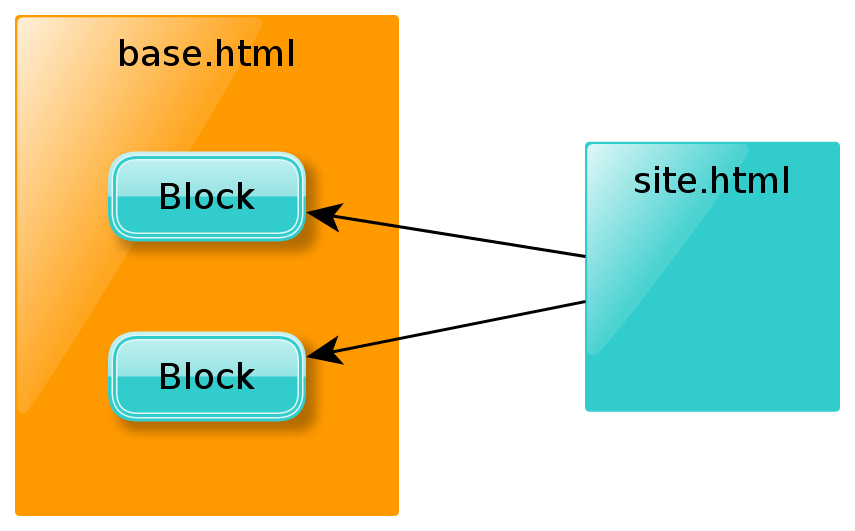
\includegraphics[width=\textwidth] {template.png}
      \end{figure}
    \end{column}
\end{columns}

\end{frame}


\begin{frame}[fragile]
    \frametitle{Templates}
    \framesubtitle{Cheetah}
     \begin{itemize}[<1->]
        \item Wird von allen Full-Stack-Frameworks unterstützt
        \item Große und aktive Community
        \item Templates können von Python-Klassen abgeleitet werden
     \end{itemize}
\begin{lstlisting}
<table>
   #for $client in $clients
      <tr>
         <td>$client.surname, $client.firstname</td>
         <td><a href="mailto:$client.email">$client.email</a></td>
      </tr>
   #end for
</table>
\end{lstlisting}
\end{frame}


\begin{frame}[fragile]
  \frametitle{I18N und L10N}
  \framesubtitle{Django}
  \begin{itemize}[<1->]
    \item Unterstützt Textübersetzung, Datums-, Zeit und Zahlenformattierung, Zeitzonen und Pluralisierung
    \item Markieren der Texte mit ugettext
  \end{itemize}
  \begin{lstlisting}
   from django.utils.translation import ugettext as _

   def my_view(request):
      output = _("Welcome to my site.")
      return HttpResponse(output)
  \end{lstlisting}
  \begin{itemize}[<1->]
    \item Werkzeuge zum erstellen neuer Sprachdateien: \\
        \textbf{django-admin.py makemessages -l de}
  \end{itemize}
   \begin{lstlisting}
   #: path/to/python/module.py:23
   msgid "Welcome to my site."
   msgstr ""
   \end{lstlisting}
\end{frame}
\begin{frame}
  \frametitle{I18N und L10N}
  \framesubtitle{Turbogears 2.0}
  \begin{itemize}[<1->]
    \item Internationalisierung mit Python Modul \textit{gettext}
    \item Funktionsweise analog zu Django
    \item .po-Sprachdateien können auch mit Hilfsmitteln bearbeitet werden
  \end{itemize}
  \begin{figure}
        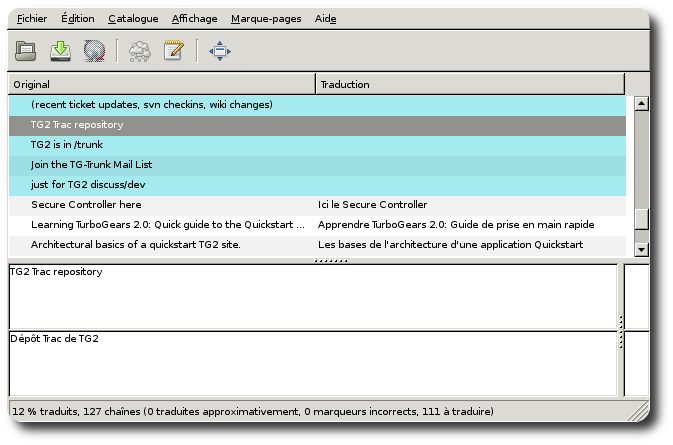
\includegraphics[height=55mm] {poedit.png}
        \source{[\ref{illu:8}]}
      \end{figure}
\end{frame}

\begin{frame}
  \frametitle{Routing}
    Django
    \begin{itemize}[<1->]
        \item URLconf (URL Konfiguration)
        \item einfaches Mapping zwischen URL-Patterns (Regex)
        \item Wenn der Ausdruck passt, ruft Django den View auf
        \item settings.py für alle weiteren Konfigurationen
        \begin{itemize}[<1->]
            \item Datenbankeinstellungen
            \item E-Mail und Fehlermeldungseinstellungen
            \item i18n und URL Einstellungen
            \item Applikations and Middleware Einstellungen
        \end{itemize}
     \end{itemize}

\end{frame}

\begin{frame}[fragile]
\frametitle{Routing Beispiel Django}
\begin{lstlisting}
urlpatterns = patterns('news.views',
    (r'^articles/2003/$', 'special_case_2003'),
    (r'^articles/(\d{4})/$', 'year_archive'),
    (r'^articles/(\d{4})/(\d{2})/$', 'month_archive'),
    (r'^articles/(\d{4})/(\d{2})/(\d+)/$', 'article_detail'),
)
\end{lstlisting}
\hrule
\begin{lstlisting}
/articles/2005/03/     => month_archive(request,'2005','03')
/articles/2005/3/      => no match
/articles/2003/        => special_case_2003(request,'2003')
/articles/2003         => no match
/articles/2003/03/03/  => article_detail(request,'2003','03','03')
    \end{lstlisting}
\end{frame}


\begin{frame}
  \frametitle{Routing}
TurboGears

\begin{beamerpostit}
    \begin{quote}
      “\dots By default you don’t need to think about Routes at all \dots”
    \end{quote} %~ FIXME Quelle
  \end{beamerpostit}

     \begin{itemize}[<1->]
        \item Object Dispatch, und built in Routes Integration
        \item kann überschrieben werden
        \item Verwendet Routes (Python Implementierung des Rails-Routes-System)
    \end{itemize}
\end{frame}


\begin{frame}[fragile]
\frametitle{Routing Beispiel TurboGear 2.0}

\end{frame}

\begin{frame}
    \frametitle{Routing}

    \todo{Wie messen Sie "mächtig" und "einfach"?}
    \begin{table}[h]
        \begin{tabular}{|c|c|c|}
            \hline
             & Django & TurboGear 2.0  \\ \hline
            Routing & \cellcolor{dkgreen} mächtig & \cellcolor{dkgreen} einfach,anpassbar     \\ \hline
         \end{tabular}
    \end{table}
\end{frame}


\begin{frame}
  \frametitle{Sicherheitmechanismen}

  \begin{itemize}[<1->]
    \item django: http://www.djangobook.com/en/2.0/chapter20.html
    \end{itemize}

\end{frame}


\begin{frame}[fragile]
  \frametitle{Bootstrapping, Scaffolding, Erweiterbarkeit}
Django
 \begin{itemize}[<1->]
    \item django-common-helpers plugin (https://github.com/Tivix/django-common)
    \item create app,create models,create views,create templates,create forms,create urls,create tests.
    \item Generic-Views
 \end{itemize}
    \vspace{15pt}


\end{frame}


\begin{frame}
  \frametitle{Extras: WebServices, Caching, Tests}
\end{frame}


\section{noch mehr Frameworks ;-)}

%~ Why use microframework?
%~ Single Codebases are great
%~ Single codebases are EVIL!
%~ http://pydanny-event-notes.readthedocs.org/en/latest/DjangoConEurope2012/flasky-goodness-or-why-django-sucks.html

\begin{frame}
  \frametitle{Flask}
  %~ http://en.wikipedia.org/wiki/Flask_%28programming%29
  %~ http://www.slideshare.net/trustrachel/django-vs-flask

  \vspace{-4pt}
  \begin{beamerpostit}
    \begin{quote}
      “\dots microframework for Python based on Werkzeug, Jinja2 and good intentions\dots”
    \end{quote} %~ FIXME Quelle
  \end{beamerpostit}

    \begin{columns}<1->
            \begin{column}{.6\textwidth}<1->
            \begin{itemize}[<1->]
                    \item Flexibilität für Entwickler%
                    % wenig Einschränkungen/Vorschriften bei Quelltext
                    % Anwendungsarchitektur nach eigenem Geschmack
                    % freie Komponentenwahl, keine überflüssigen Komponenten
                    \item Entwicklungsserver und Debugger
                    \item Unittest-Unterstützung
                    \item RESTful
                    \item Template-Sprache Jinja2
                    %\item Secure-Cookies
                    %\item WSGI 1.0 konform
                    \item inspiriert von Sinatra (Ruby)
            \end{itemize}
            \end{column}

    \begin{column}{.4\textwidth}<1->
            \begin{figure}
                    
\includegraphics[width=\textwidth]{flask_logo.png}
                    \source{[\ref{illu:3}]}
                \end{figure}
            \end{column}

        \end{columns}
\end{frame}


\begin{frame}[fragile]
  \frametitle{Flask}
  \framesubtitle{Minimalbeispiel einer Webanwendung}

  \vspace{-12pt}
  \begin{lstlisting}[title=hello.py]
from flask import Flask

app = Flask(__name__)

@app.route('/')
def hello_world():
    return 'Hello World!'

if __name__ == '__main__':
    app.run()
  \end{lstlisting}
  \hrule
  \begin{lstlisting}
$ python hello.py
* Running on http://127.0.0.1:5000/
  \end{lstlisting}%~$
\end{frame}


\begin{frame}

 \begin{columns}[T]<1->

 	\begin{column}{.3\textwidth}<1->
            
    		\begin{figure}
        		
\includegraphics[width=100px]{tornado_logo.png}
                    \source{[\ref{illu:4}]}
                \end{figure}
	\end{column}                
  %~ http://en.wikipedia.org/wiki/Tornado_%28web_server%29
  %~ http://developers.facebook.com/blog/post/301/
  %~ http://news.cnet.com/8301-17939_109-10349836-2.html

 \begin{column}{.6\textwidth}<1->
            
  \vspace{15px}
  \begin{beamerpostit}
    \begin{quote}
      “\dots FriendFeed’s web server is a relatively simple, non-blocking web
      server written in Python\dots Tornado is an open source version of this web
      server and some of the tools we use most often at FriendFeed\dots”
    \end{quote} %~ FIXME Quelle
  \end{beamerpostit}
  \end{column}
  \end{columns}
  
\vspace{20px}
   \begin{itemize}[<1->]
   		\item Webframework und Webserver für Python
   \end{itemize}

   \begin{figure}
   		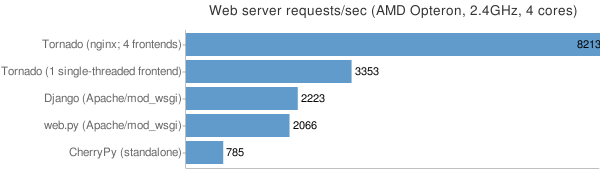
\includegraphics[width=\textwidth]{tornado_stat.png}
         \source{[\ref{illu:5}]}
   \end{figure}

\end{frame}


\begin{frame}[fragile]

  \frametitle{Tornado}
  \framesubtitle{Minimalbeispiel einer Webanwendung}

  \vspace{-12pt}
  \begin{lstlisting}[title=hello.py]
from tornado import ioloop, web

class MainHandler(web.RequestHandler):
    def get(self):
        self.write("Hello, world")

application = web.Application([
    (r"/", MainHandler),
])

if __name__ == "__main__":
    application.listen(8888)
    ioloop.IOLoop.instance().start()
    \end{lstlisting}
\end{frame}

\begin{frame}
    \begin{columns}[T]

            \begin{column}{.3\textwidth}<1->
            \begin{figure}
                    
\includegraphics[width=25mm]{bottle_logo.png}
                    \source{[\ref{illu:6}]}
                \end{figure}

                "...a fast, simple and lightweight WSGI micro web-framework for Python."
            \end{column}


            \begin{column}{.7\textwidth}<1->
            \vspace{100px}
            \begin{itemize}[<1->]
                \item Was kann/ist Bottle ?
            \begin{itemize}[<1->]
                    \item Routing - saubere und dynamische URLs
                    \item Eingebaute Template-Engine (unterstützt auch mako, jinja2 und cheetah)
                    \item Formular-Daten Zugriff, Dateiuploads, Cookies,...
                    \item Eingebauter Entwicklungsserver

                \end{itemize}
        \end{itemize}

            \end{column}

        \end{columns}
\end{frame}

\begin{frame}[fragile]
  \frametitle{Bottle Beispiel}

  \begin{lstlisting}
from bottle import route, run, template

@route('/hello/:name')
def index(name='World'):
    return template('<b>Hello {{name}}</b>!', name=name)

run(host='localhost', port=8080)

\end{lstlisting}
\end{frame}



\begin{frame}

    \begin{columns}[T]

            \begin{column}{.3\textwidth}<1->
            \begin{figure}
                    
\includegraphics[width=25mm]{webpy_logo.png}
                    \source{[\ref{illu:7}]}
                \end{figure}

                "...is a web framework for Python that is as simple as it is powerful..."
            \end{column}


            \begin{column}{.7\textwidth}<1->
            \vspace{100px}
            \begin{itemize}[<1->]
                \item Was kann/ist web.py ?
            \begin{itemize}[<1->]
                    \item ...
                \end{itemize}
        \end{itemize}

            \end{column}

        \end{columns}
\end{frame}

\begin{frame}[fragile]
  \frametitle{web.py Beispiel}


  \begin{lstlisting}
import web

urls = (
    '/(.*)', 'hello'
)
app = web.application(urls, globals())

class hello:
    def GET(self, name):
        if not name:
            name = 'World'
        return 'Hello, ' + name + '!'

if __name__ == "__main__":
    app.run()

    \end{lstlisting}
\end{frame}

\begin{frame}
  \frametitle{Vergleich der Microframeworks}

    \begin{table}[h]
        \begin{tabular}{|c|c|c|c|c|}
            \hline
             		& Flask & Tornado & Bottle & web.py \\ \hline
            St\"arke &   &	schnell  &   &      \\ \hline
            Grenzen &   &   &   &      \\ \hline
            ?? &   &   &   &      \\ \hline
            ?? &   &   &   &      \\ \hline
            ?? &   &   &   &      \\ \hline
            ?? &   &   &   &      \\ \hline

         \end{tabular}
    \end{table}

\end{frame}

\begin{frame}
  \frametitle{Kriterienübersicht}
 * Vergleichstabellen (Django vs. ...)

    \begin{table}[h]
        \begin{tabular}{|c|c|c|}
            \hline
             & Django & TurboGear 2.0  \\ \hline
            Persistenz &   &      \\ \hline
            Formulare,Validierung &   &      \\ \hline
            Templates &   &      \\ \hline
            Routing &   &      \\ \hline
            Sicherheitsmechanismen &   &      \\ \hline
            Bootstrapping,Scaffolding &   &      \\ \hline

         \end{tabular}
    \end{table}

\end{frame}


%~ „Letzte Folie“: einprägsame Botschaft
%~ ggf. Bezug auf Eingangsfolie nehmen
\section{Fazit}
\begin{frame}
  \frametitle{Fazit}

  Je Anforderungen an das Webframework (“Taste”)\\
  \dots

  %~ * Ich hoffe, habt jetzt einen besseren Eindruck über Webframeworks für
  %~   Python gewinnen können.
  %~ * Vielen Dank für die Aufmerksamkeit.
  %~ * offene Fragen?/Diskussion genannter Punkte
  %~ * danach Kritik/Anregungen
\end{frame}


%~ Hinweise zu weiteren Informationen im Internet: die Chance, dass sich die
%~ Zuhörer das Thema Ihres Vortrags nachhaltig einprägen.
\begin{frame}
  \frametitle{Quellen}

  {\footnotesize

  %\printbibliography
  \begin{itemize}[<1->]
    \item \url{http://www.infoworld.com/d/application-development/pillars-python-six-python-web-frameworks-compared-169442}
    \item \url{http://wiki.python.org/moin/WebFrameworks}
    \item \url{http://wiki.python-forum.de/Web-Frameworks}
    \item \url{http://blog.ianbicking.org/turbogears-and-pylons.html}
    \item \url{https://docs.djangoproject.com/en/dev/topics/}
    \item \url{https://docs.djangoproject.com/en/dev/misc/design-philosophies/}
  \end{itemize}

  alle URLs aufgerufen am 20. November 2012.
  }
\end{frame}


\begin{frame}
  \frametitle{Quellen der Abbildungen}
  \footnotesize
  \begin{enumerate}[<1->]
    \item Innenhof Informatik
        \url{http://www.flickr.com/photos/bennybenny/3597853896/}       \label{illu:1}

   \item Flask Logo
        \url{http://flask.pocoo.org/static/logo.png}                    \label{illu:3}

    \item Tornado Logo
                \url{http://www.tornadoweb.org/static/tornado.png}              \label{illu:4}

    \item Tornado Statistik (Bret Taylor, 10. September 2009)
        \url{http://http://developers.facebook.com/blog/post/301/}      \label{illu:5}

    \item Bottle Logo
        \url{http://bottlepy.org/docs/dev/_static/logo_nav.png}             \label{illu:6}

    \item web.py Logo
        \url{http://webpy.org/static/webpy.gif}             \label{illu:7}
     \item po-Editor
        \url{http://www.turbogears.org/2.1/docs/_images/poedit.png}     \label{illu:8}
\item Django Logo
        \url{https://www.djangoproject.com/m/img/logos/django-logo-positive.png  }
        \label{illu:9}
  \end{enumerate}
  alle URLs aufgerufen am 14. November 2012.
\end{frame}

\end{document}
